\documentclass{article}
\usepackage{graphicx, tikz-cd, float, titlepic, booktabs} % Required for inserting images
\usepackage{pgfplots}
\pgfplotsset{compat=1.15}
\usepackage{mathrsfs}
\usetikzlibrary{arrows}
\usepackage{amsmath, amssymb, amsthm, amsfonts, siunitx, physics, gensymb}
\AtBeginDocument{\RenewCommandCopy\qty\SI}
\usepackage[version=4]{mhchem}
\usepackage[most,many,breakable]{tcolorbox}
\usepackage{xcolor, fancyhdr, varwidth}
\usepackage[Glenn]{fncychap}
%Options: Sonny, Lenny, Glenn, Conny, Rejne, Bjarne, Bjornstrup
\usepackage{hyperref, cleveref}
\usepackage{icomma, enumitem} %comma as decimal and continue enumerate with [resume]
\usepackage[danish]{babel}
%%%%%%%%%%%%%%%%%%%%%%%%%%%%%%
% SELF MADE COLORS
%%%%%%%%%%%%%%%%%%%%%%%%%%%%%%
\definecolor{myg}{RGB}{56, 140, 70}
\definecolor{myb}{RGB}{45, 111, 177}
\definecolor{myr}{RGB}{199, 68, 64}
\definecolor{mytheorembg}{HTML}{F2F2F9}
\definecolor{mytheoremfr}{HTML}{00007B}
\definecolor{mylenmabg}{HTML}{FFFAF8}
\definecolor{mylenmafr}{HTML}{983b0f}
\definecolor{mypropbg}{HTML}{f2fbfc}
\definecolor{mypropfr}{HTML}{191971}
\definecolor{myexamplebg}{HTML}{F2FBF8}
\definecolor{myexamplefr}{HTML}{88D6D1}
\definecolor{myexampleti}{HTML}{2A7F7F}
\definecolor{mydefinitbg}{HTML}{E5E5FF}
\definecolor{mydefinitfr}{HTML}{3F3FA3}
\definecolor{notesgreen}{RGB}{0,162,0}
\definecolor{myp}{RGB}{197, 92, 212}
\definecolor{mygr}{HTML}{2C3338}
\definecolor{myred}{RGB}{127,0,0}
\definecolor{myyellow}{RGB}{169,121,69}
\definecolor{myexercisebg}{HTML}{F2FBF8}
\definecolor{myexercisefg}{HTML}{88D6D1}
%%%%%%%%%%%%%%%%%%%%%%%%%%%%%%%%%%%%%%%%%%%%%%%%%%%%%%%%%%%%%%%%%%%%%%
% Box environments for theorems and problems
%%%%%%%%%%%%%%%%%%%%%%%%%%%%%%%%%%%%%%%%%%%%%%%%%%%%%%%%%%%%%%%%%%%%%
\setlength{\parindent}{1cm}
%================================
% Question BOX
%================================
\makeatletter
\newtcbtheorem{question}{Opgave}{enhanced,
	breakable,
	colback=white,
	colframe=myb!80!black,
	attach boxed title to top left={yshift*=-\tcboxedtitleheight},
	fonttitle=\bfseries,
	title={#2},
	boxed title size=title,
	boxed title style={%
			sharp corners,
			rounded corners=northwest,
			colback=tcbcolframe,
			boxrule=0pt,
		},
	underlay boxed title={%
			\path[fill=tcbcolframe] (title.south west)--(title.south east)
			to[out=0, in=180] ([xshift=5mm]title.east)--
			(title.center-|frame.east)
			[rounded corners=\kvtcb@arc] |-
			(frame.north) -| cycle;
		},
	#1
}{def}
\makeatother
%================================
% DEFINITION BOX
%================================

\newtcbtheorem[]{Definition}{Definition}{enhanced,
	before skip=2mm,after skip=2mm, colback=red!5,colframe=red!80!black,boxrule=0.5mm,
	attach boxed title to top left={xshift=1cm,yshift*=1mm-\tcboxedtitleheight}, varwidth boxed title*=-3cm,
	boxed title style={frame code={
					\path[fill=tcbcolback]
					([yshift=-1mm,xshift=-1mm]frame.north west)
					arc[start angle=0,end angle=180,radius=1mm]
					([yshift=-1mm,xshift=1mm]frame.north east)
					arc[start angle=180,end angle=0,radius=1mm];
					\path[left color=tcbcolback!60!black,right color=tcbcolback!60!black,
						middle color=tcbcolback!80!black]
					([xshift=-2mm]frame.north west) -- ([xshift=2mm]frame.north east)
					[rounded corners=1mm]-- ([xshift=1mm,yshift=-1mm]frame.north east)
					-- (frame.south east) -- (frame.south west)
					-- ([xshift=-1mm,yshift=-1mm]frame.north west)
					[sharp corners]-- cycle;
				},interior engine=empty,
		},
	fonttitle=\bfseries,
	title={#2},#1}{def}
\newtcbtheorem[]{definition}{Definition}{enhanced,
	before skip=2mm,after skip=2mm, colback=red!5,colframe=red!80!black,boxrule=0.5mm,
	attach boxed title to top left={xshift=1cm,yshift*=1mm-\tcboxedtitleheight}, varwidth boxed title*=-3cm,
	boxed title style={frame code={
					\path[fill=tcbcolback]
					([yshift=-1mm,xshift=-1mm]frame.north west)
					arc[start angle=0,end angle=180,radius=1mm]
					([yshift=-1mm,xshift=1mm]frame.north east)
					arc[start angle=180,end angle=0,radius=1mm];
					\path[left color=tcbcolback!60!black,right color=tcbcolback!60!black,
						middle color=tcbcolback!80!black]
					([xshift=-2mm]frame.north west) -- ([xshift=2mm]frame.north east)
					[rounded corners=1mm]-- ([xshift=1mm,yshift=-1mm]frame.north east)
					-- (frame.south east) -- (frame.south west)
					-- ([xshift=-1mm,yshift=-1mm]frame.north west)
					[sharp corners]-- cycle;
				},interior engine=empty,
		},
	fonttitle=\bfseries,
	title={#2},#1}{def}

\newtcbtheorem{theo}%
    {Theorem}{}{theorem}
\newtcolorbox{prob}[1]{colback=red!5!white,colframe=red!50!black,fonttitle=\bfseries,title={#1}}
%================================
% NOTE BOX
%================================

\usetikzlibrary{arrows,calc,shadows.blur}
\tcbuselibrary{skins}
\newtcolorbox{note}[1][]{%
	enhanced jigsaw,
	colback=gray!20!white,%
	colframe=gray!80!black,
	size=small,
	boxrule=1pt,
	title=\textbf{Note:},
	halign title=flush center,
	coltitle=black,
	breakable,
	drop shadow=black!50!white,
	attach boxed title to top left={xshift=1cm,yshift=-\tcboxedtitleheight/2,yshifttext=-\tcboxedtitleheight/2},
	minipage boxed title=1.5cm,
	boxed title style={%
			colback=white,
			size=fbox,
			boxrule=1pt,
			boxsep=2pt,
			underlay={%
					\coordinate (dotA) at ($(interior.west) + (-0.5pt,0)$);
					\coordinate (dotB) at ($(interior.east) + (0.5pt,0)$);
					\begin{scope}
						\clip (interior.north west) rectangle ([xshift=3ex]interior.east);
						\filldraw [white, blur shadow={shadow opacity=60, shadow yshift=-.75ex}, rounded corners=2pt] (interior.north west) rectangle (interior.south east);
					\end{scope}
					\begin{scope}[gray!80!black]
						\fill (dotA) circle (2pt);
						\fill (dotB) circle (2pt);
					\end{scope}
				},
		},
	#1,
}

%%%%%%%%%%%%%%%%%%%%%%%%%%%%%%%%%%%%%%%%%%%%%%%%%%%%%%%%%%%%%%%%%
% SELF MADE COMMANDS
%%%%%%%%%%%%%%%%%%%%%%%%%%%%%%
\newcommand{\sol}{\setlength{\parindent}{0cm}\textbf{\textit{Løsning:}}\setlength{\parindent}{1cm}}
%%%%%%%%%%%%%%%%%%%%%%%%%%%%%%%%%
\usepackage[tmargin=2cm,rmargin=1in,lmargin=1in,margin=0.85in,bmargin=2cm,footskip=.2in]{geometry}\pagestyle{fancy}
\lhead{Minrui Kevin Zhou 2.b}
\rhead{Matematikaflevering 24}

\title{Aflevering 24\\
{\Large \textbf{2.b mat A}}}
\author{Kevin Zhou}
\date{Februar 2024}

\begin{document}
\maketitle
\section*{Bedømmelseskriterier:}
\begin{itemize}
    \setlength\itemsep{3cm}
    \Large
    \item  Redegørelse og dokumentation for metode
    \item Figurer, grafer og andre illustrationer
    \item Notation og layout
    \item Formidling og forklaring
\end{itemize}
\pagebreak

\begin{question}{}{}
  I planen er der givet to vektorer, $\va{a} =\begin{pmatrix} t-2\\ 5 \end{pmatrix}$ og $\va{b} =\begin{pmatrix} 3\\ -3 \end{pmatrix},\quad t \in \mathbb{R} $. \\
Bestem tallet $t$, så vektorerne $\va{a} $ og $\va{b} $ er ortogonale. 
\end{question}
\sol \\ 
Når vektorerne er ortogonale, så må dotproduktet være lig med 0.
\begin{equation*}
\begin{split}
  \va{a} \perp \va{b} &\iff \va{a} \cdot \va{b} =0\\ 
  &\iff 3 \cdot \left(t-2\right) + 5 \cdot \left(-3\right) =0\\ 
  &\iff 3t=21\\ 
  &\iff t=7
\end{split}
\end{equation*}
\begin{question}{}{}
  Bestem $t \in \mathbb{R}$ sådan at vektorerne $\va{a} = \begin{pmatrix} 2\\ 2t-3 \end{pmatrix} $ og $\va{b} =\begin{pmatrix} 4\\ 7t-5 \end{pmatrix} $ er parallelle. 
\end{question}
\sol \\ 
Når vektorerne er parallelle, så må determinanten være lig med 0.
\begin{equation*}
\begin{split}
  \va{a} \parallel \va{b} &\iff \mdet{2 & 4 \\ 2t-3 & 7t-5} = 0\\ 
  &\iff 14t-10-8t+12=0 \\ 
  &\iff 6t=-2\\ 
  &\iff t=-\frac{1}{3}
\end{split}
\end{equation*}
\begin{question}{}{}
 I et koordinatsystem er to vektorer $\va{a} $ og $\va{b} $ givet ved 
  \[
  \va{a} =\begin{pmatrix} 3\\ 2 \end{pmatrix} \text{ og } \va{b}=\mqty(-2\\ 5) 
  \] 
  Bestem arealet af det parallelogram, som $\va{a} \text{ og }\va{b} $ udspænder 
\end{question}
\sol \\
Arealet af parallelogrammet er den absolutte værdi af determinanten for de to vektorer.
\begin{equation*}
\begin{split}
  A&=\left| \mdet{3 & -2 \\ 2 & 5}  \right| \\ 
  &=\left| 15 -2 \cdot \left(-2\right) \right| \\ 
  &=19
\end{split}
\end{equation*}
Altså er arealet af parallelogrammet 19.
\begin{question}{}{}
  En indhegning har form som vist på figuren i pdf-filen i lectio.
  Nogle af målene er angivet på figuren.
  \begin{itemize}
    \item[a.] Indlæg en model af indhegningen i et koordinatsystem, hvor koordinatsættet for punktet $A$ er $(0,0)$. 
    \item[b.] Bestem koordinatsættene for vektorerne $\overrightarrow{\textbf{CB}} \text{ og } \overrightarrow{\textbf{CD}} $ i min model. 
    \item[c.] Beregn indhegningens omkreds.
  \end{itemize}
\end{question}
\sol \\
\textbf{a.} 
En model af indhegningen i et koordinatsystem kan ses i \cref{fig:indhegning}.
\begin{figure}[H]
\begin{center}
\definecolor{zzttqq}{rgb}{0.6,0.2,0.}
\definecolor{ududff}{rgb}{0.30196078431372547,0.30196078431372547,1.}
\definecolor{xdxdff}{rgb}{0.49019607843137253,0.49019607843137253,1.}
\definecolor{uuuuuu}{rgb}{0.26666666666666666,0.26666666666666666,0.26666666666666666}
\begin{tikzpicture}[line cap=round,line join=round,>=triangle 45,x=1.0cm,y=1.0cm]
\begin{axis}[
x=1.0cm,y=1.0cm,
axis lines=middle,
ymajorgrids=true,
xmajorgrids=true,
xmin=-1.0,
xmax=10.0,
ymin=-1.0,
ymax=11.0,
xtick={-0.0,2.0,...,10.0},
ytick={-0.0,2.0,...,10.0},]
\clip(-1.,-1.) rectangle (10.,11.);
\fill[line width=2.pt,color=zzttqq,fill=zzttqq,fill opacity=0.10000000149011612] (0.,0.) -- (8.,0.) -- (8.,4.) -- (0.,10.) -- cycle;
\draw [line width=2.pt,color=zzttqq] (0.,0.)-- (8.,0.);
\draw [line width=2.pt,color=zzttqq] (8.,0.)-- (8.,4.);
\draw [line width=2.pt,color=zzttqq] (8.,4.)-- (0.,10.);
\draw [line width=2.pt,color=zzttqq] (0.,10.)-- (0.,0.);
\begin{scriptsize}
\draw [fill=uuuuuu] (0.,0.) circle (2.0pt);
\draw[color=uuuuuu] (0.18441683895061886,0.4371977496058456) node {$A$};
\draw [fill=xdxdff] (8.,0.) circle (2.5pt);
\draw[color=xdxdff] (8.173017458079237,0.4894108255478628) node {$B$};
\draw [fill=ududff] (8.,4.) circle (2.5pt);
\draw[color=ududff] (8.173017458079237,4.483711135112175) node {$C$};
\draw [fill=xdxdff] (0.,10.) circle (2.5pt);
\draw[color=xdxdff] (0.18441683895061886,10.488214868444148) node {$D$};
\draw[color=zzttqq] (3.943758306775851,-0.7898095350315576) node {$8$};
\draw[color=zzttqq] (8.48629591373134,2.2385488696054376) node {$4$};
\draw[color=zzttqq] (-0.7554185280056891,5.084161508445373) node {$10$};
\end{scriptsize}
\end{axis}
\end{tikzpicture}
\end{center}
\caption{Model tegnet med GeoGebra og TikZ}
\label{fig:indhegning}
\end{figure}
\noindent \textbf{b.}
Koordinatsættene for $\overrightarrow{\textbf{CB}} \text{ og } \overrightarrow{\textbf{CD}} $ er da 
\begin{equation*}
\begin{split}
  \overrightarrow{\textbf{CB}} &=\mqty(0\\ -4) \\ 
  \overrightarrow{\textbf{CD}} &=\mqty(-8\\ 6) 
\end{split}
\end{equation*}
\textbf{c.}
Indhegningens omkreds er da summen af længden af de tre angivne sider og længden af $\overrightarrow{\textbf{CD}} $.
\begin{equation*}
\begin{split}
  O&=10+8+4+\left| \overrightarrow{\textbf{CD}}  \right| \\ 
  &=22+\sqrt{\left(-8\right)^2+6^2} \\ 
  &= 32
\end{split}
  \end{equation*}
Altså er indhegningens omkreds 32.
\begin{question}{}{}
  Fotoet (\cref{fig:foto}) viser et træ, som vinden har fået til at hælde.
  Der er indlagt et koordinatsystem på fotoet.
  Den vandrette afstand fra $O$ til punktet $B$ på jorden er $0,60 \;\unit{m} $.
  Den lodrette aftand fra $B$ til punktet $A$ er $2,25 \;\unit{m} $.
  \begin{itemize}
    \item[a.] Bestem koordinatsættene til vektorerne $\overrightarrow{\textbf{OA}} \text{ og } \overrightarrow{\textbf{OB}} $.
    \item[b.] Bestem vinkel $v$.
  \end{itemize}
\end{question}
\begin{figure}[H]
\begin{center}
  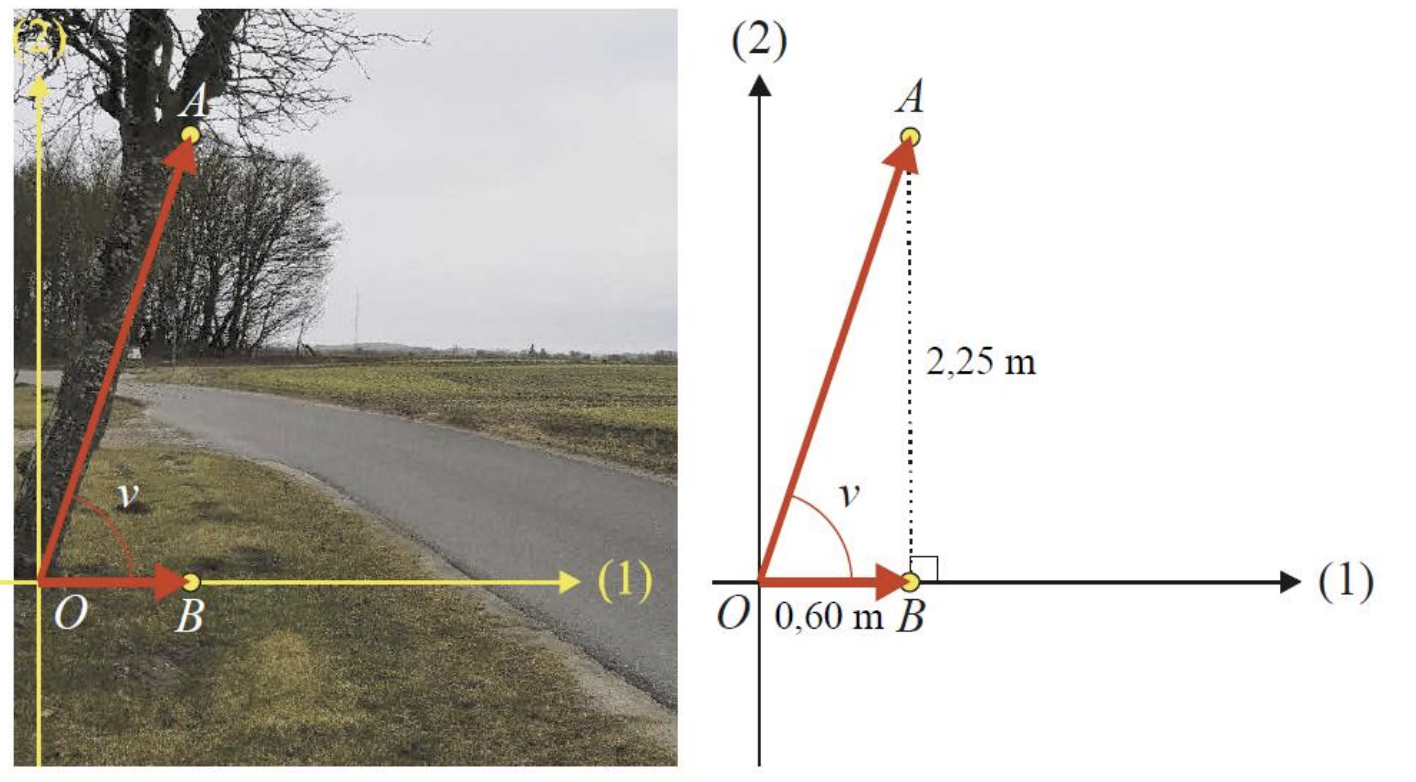
\includegraphics[scale=0.5]{foto.png}
\end{center}
\caption{Fotoet}
\label{fig:foto}
\end{figure}
\sol \\
\textbf{a.}
Koordinatsættene til $\overrightarrow{\textbf{OA}} \text{ og } \overrightarrow{\textbf{OB}} $ er da
\begin{equation*}
\begin{split}
  \overrightarrow{\textbf{OA}} &=\mqty(0,6\\ 2,25) \\ 
  \overrightarrow{\textbf{OB}} &=\mqty(0,6\\ 0) 
\end{split}
\end{equation*}
\textbf{b.} 
Vi bestemmer $v$ med de to vektorer fra \textbf{a.}. 
\begin{equation*}
\begin{split}
  v&=\cos^{-1}\left(\frac{\overrightarrow{\textbf{OA}} \cdot \overrightarrow{\textbf{OB}} }{\left| \overrightarrow{\textbf{OA}} \right|\cdot \left|\overrightarrow{\textbf{OB}}   }  \right| \right) \\ 
  &=\cos^{-1}\left(\frac{0,6^2}{\sqrt{0,6^2 \cdot \left(0,6^2+2,25^2\right) } }\right) \\ 
  &\approx 75 \degree 
\end{split}
\end{equation*}
Altså er vinklen $v$ cirka $75 \degree $. 
\end{document}
